\section{Problem and data description}
\label{sec:data}

\subsection{Task and research question}
The task is supervised image classification: assign one clothing category to
each image. Category prediction can help organize online product catalogs.
The study asks how linear, multilayer, convolutional, recurrent, and Transformer
models differ in accuracy and class confusions on the same data splits.

For Fashion-MNIST, the model receives a normalized grayscale tensor
$x\in\mathbb{R}^{1\times28\times28}$ and returns ten class scores
$f_\theta(x)\in\mathbb{R}^{10}$. Its prediction is
$\hat y=\arg\max_{k\in\{0,\ldots,9\}} f_\theta(x)_k$.
The prediction unit is one image. Low resolution and similar garment outlines
make some categories difficult to separate.

\subsection{Dataset and study scope}
Fashion-MNIST contains 70,000 Zalando product images with supplied category
labels: 60,000 official training images and 10,000 official test images
\cite{fashionmnist}. Labels 0--9 denote T-shirt/top, Trouser, Pullover, Dress,
Coat, Sandal, Shirt, Sneaker, Bag, and Ankle boot, respectively.

We use the standard IDX distribution from the authors' MIT-licensed repository
\cite{fashionmnist-data}. The four cached gzip files total 30.88 MB and match
the published MD5 checksums. Images are unsigned 8-bit arrays; labels are
integer class IDs. No samples are removed or relabelled. The small, isolated
product images and fixed category set limit how far results extend to full
scenes or unfamiliar products.

Fashion-MNIST is the main comparison dataset. MNIST handwritten digits are used
for development, and CIFAR-10 colour images provide a separate extension
\cite{mnist-data,cifar10-data}. Their roles and working splits appear in
Table~\ref{tab:data-splits}.
\begin{table}[htbp]
\centering\small
\caption{Dataset roles, native image sizes, and split counts. Image dimensions
are height $\times$ width $\times$ channels. Counts refer to images.}
\label{tab:data-splits}
\begin{tabular}{llcrrr}
\toprule
Dataset & Role & Image size & Train & Validation & Test\\
\midrule
Fashion-MNIST & Main comparison & $28\times28\times1$ & 54,000 & 6,000 & 10,000\\
MNIST & Development & $28\times28\times1$ & 54,000 & 6,000 & 10,000\\
CIFAR-10 & Extension & $32\times32\times3$ & 45,000 & 5,000 & 10,000\\
\bottomrule
\end{tabular}
\end{table}


\clearpage
\subsection{Exploratory data analysis}
\label{sec:eda}
The following statistics use the full, unaugmented official Fashion-MNIST
training set, before the train/validation split. Every image is $28\times28$
pixels. Each class has 6,000 images, so the largest-to-smallest class ratio is
1.00. The official test set has 1,000 images per class.
Figure~\ref{fig:data-samples} shows one real example per class.

\begin{figure}[H]
  \centering
  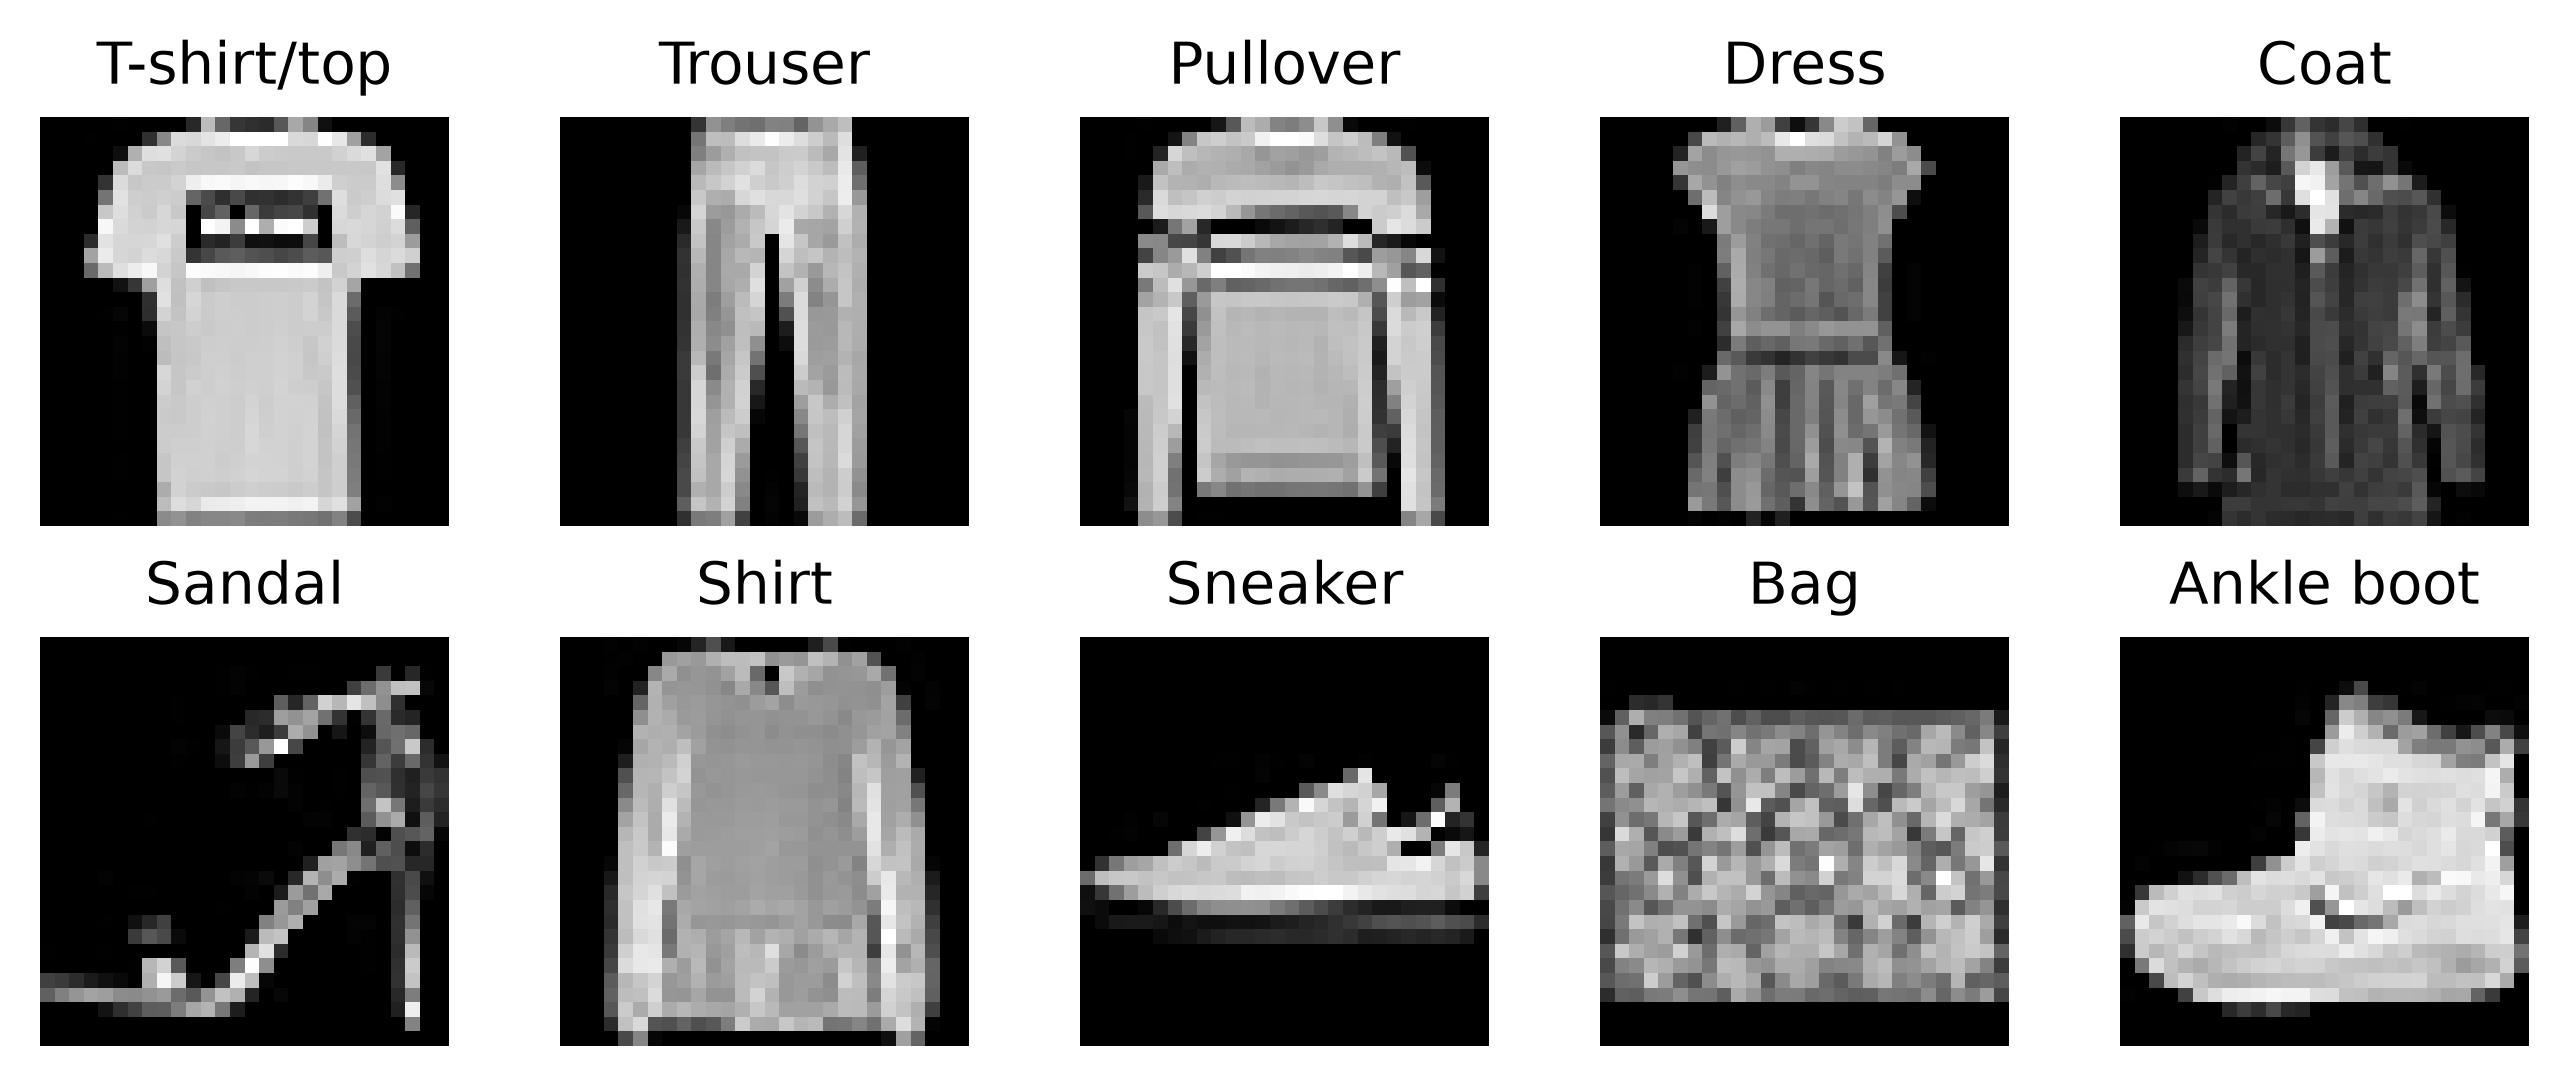
\includegraphics[width=0.90\linewidth]{Images/fashion_mnist_samples.png}
  \caption{Fashion-MNIST: the first image of each class in official training
  order, selected without using model predictions.}
  \label{fig:data-samples}
\end{figure}

Pixel intensity has mean 72.94 and standard deviation 90.02 on the 0--255 scale.
About 53.0\% of pixels fall in the lowest histogram bin (intensities 0--7),
reflecting the dark background. Defining foreground as intensity above 32 gives
average coverage from 24.5\% for Sandal to 59.8\% for Pullover.

Figure~\ref{fig:data-similarity} compares class-average images after subtracting
the average across classes. Cosine similarity is 0.86 for Pullover--Coat and
0.82 for both Sandal--Sneaker and Pullover--Shirt. These pairs motivate later
inspection of class confusions; prototype similarity does not measure model
errors.

\begin{figure}[H]
  \centering
  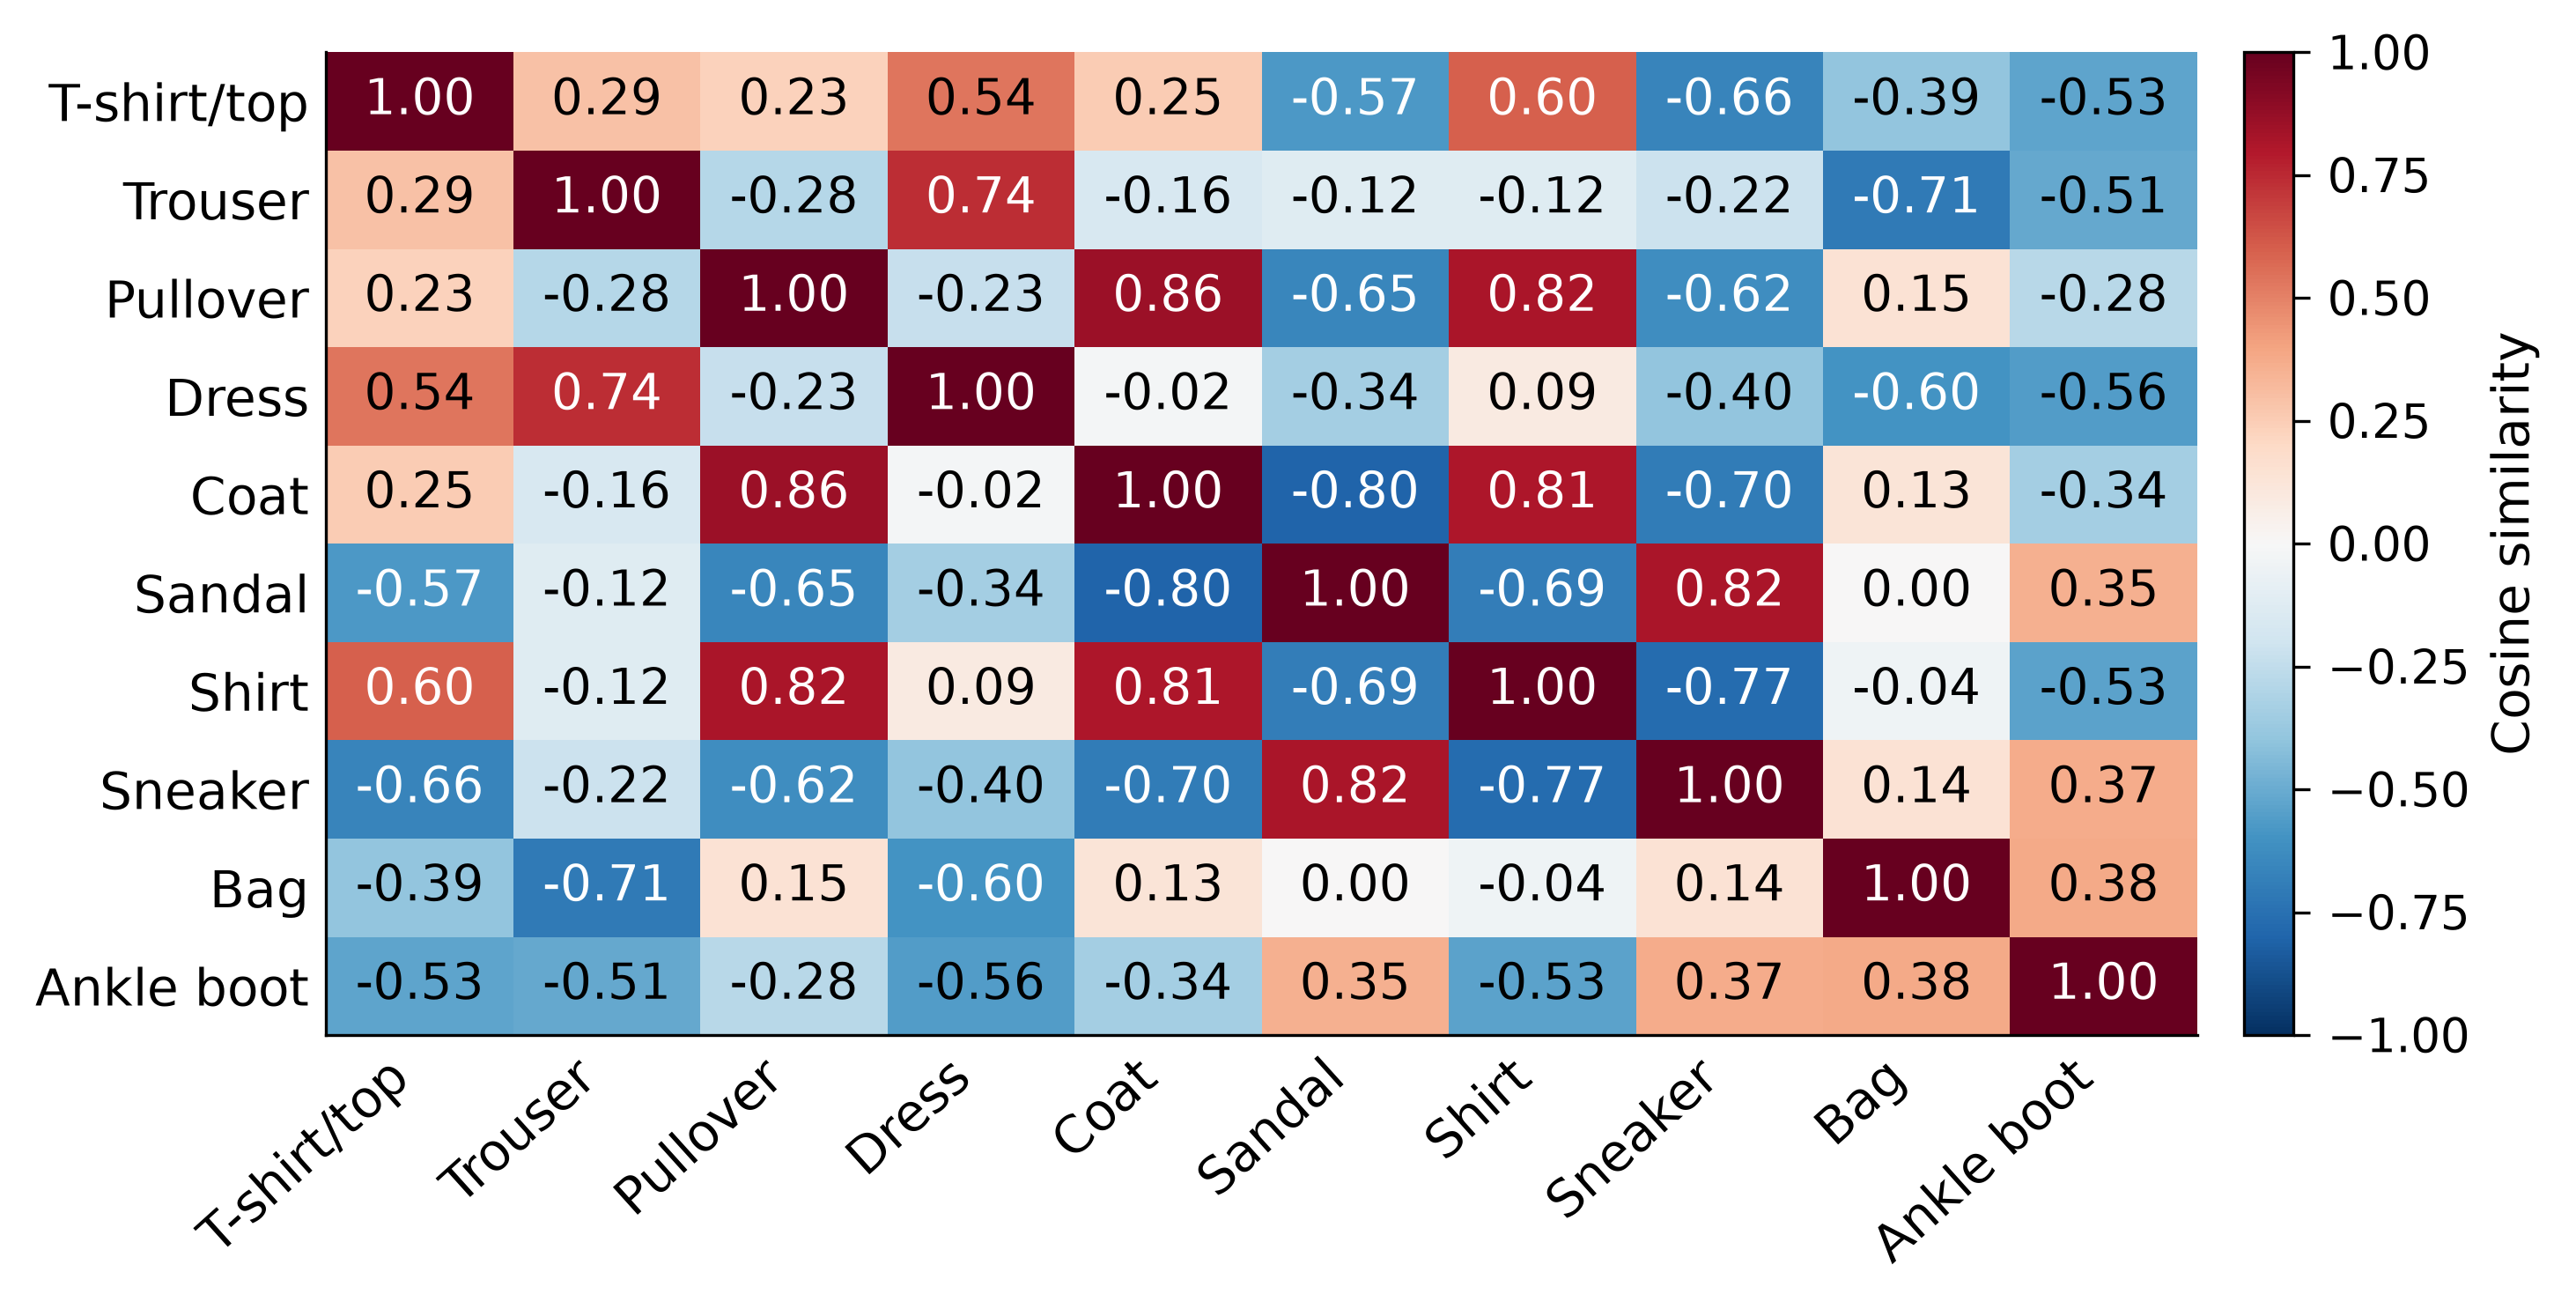
\includegraphics[width=0.90\linewidth]{Images/fashion_mnist_similarity.png}
  \caption{Cosine similarity between centred Fashion-MNIST class-average
  images, computed from the 60,000 official training images.}
  \label{fig:data-similarity}
\end{figure}

\clearpage
\subsection{Splits and leakage prevention}
\label{sec:splits}
For each dataset, a random permutation with seed 42 reserves 10\% of the official
training set for validation. The split unit is one image, and sampling is not
stratified. For Fashion-MNIST, class counts therefore range from 5,353 to 5,445
in training and from 555 to 647 in validation. All models use the same indices
for a given dataset.

The official test sets remain separate from training and validation. Validation
loss selects checkpoints; test results are reserved for reporting. Training and
validation indices are disjoint. No additional duplicate-image or product-level
audit is recorded, so this separation does not establish independence between
all images.

\subsection{Preprocessing and augmentation}
\label{sec:preprocessing}
MNIST and Fashion-MNIST keep their native resolution. Pixels are converted to
float32 in $[0,1]$, then normalized as $x'=(x-0.5)/0.5$. Training adds random
rotation within $\pm10^\circ$ and translation up to 10\% of image size.

CIFAR-10 uses four-pixel padding, a $32\times32$ random crop, and a random
horizontal flip for training. We normalize its RGB channels using mean
$(0.4914,0.4822,0.4465)$ and standard deviation $(0.2470,0.2435,0.2616)$.
Validation and test data receive conversion and normalization only.

An inspected Fashion-MNIST validation batch has float32 image shape
$[128,1,28,28]$ and values from $-1$ to $1$. Its int64 labels have shape $[128]$;
the first eight IDs are $[9,2,5,0,5,1,3,5]$. In the shared $[B,C,H,W]$ convention,
$B$ is batch size, $C$ is channels, and $H,W$ are image height and width.
CIFAR-10 batches use shape $[B,3,32,32]$.
